\section{«Build your own tools»: Entwicklung der App \textit{InterMind}}
\label{sec:entwicklung_app}

Im Zuge dieser Arbeit wurde die App \textit{InterMind} entwickelt, die als technische Grundlage für wiederholte, geolokalisierte und pseudonymisierte Befragungen dient. Sie bildet die Infrastruktur für anschliessend durchgeführte Pilot-Studie. Die App und der in dieser Arbeit eingesetzte Fragenkatalog wurden parallel und iterativ konzipiert. Während dieser Abschnitt die technische Entwicklung der App dokumentiert, wird die inhaltliche Gestaltung des Fragebogens im \cref{sec:fragebogenentwicklung} erläutert. Der vollständige Quellcode der App ist auf \gls{github}\footnote{\href{https://github.com/lbatschelet/intermind}{https://github.com/lbatschelet/intermind}} veröffentlicht.


\subsection{From scratch – Warum eine eigene App?}

Die zentrale Erhebungslogik der vorliegenden Arbeit basiert auf wiederholten, geolokalisierten Erhebungen zum situativ-affektiven Wohlbefinden der Teilnehmenden. Daraus resultieren spezifische Anforderungen an das Instrument, mit dem diese Daten erfasst werden sollen. Ein geeignetes Erhebungstool muss insbesondere folgende Kriterien erfüllen: Es soll mobil und einfach nutzbar sein, situative Antworten unmittelbar im Alltag der Teilnehmenden ermöglichen, dabei Standortdaten automatisch erfassen und gleichzeitig datenschutzrechtliche sowie technische Hürden für die Nutzer\genderstern innen minimieren. Darüber hinaus war es von Beginn an wichtig, dass das System flexibel und nachhaltig konzipiert ist, um auch für zukünftige Arbeiten eingesetzt werden zu können. Konkret bedeutet dies, dass die Fragenkataloge sowie die Inhalte der App einfach austauschbar und an neue Forschungsfragen oder Zielgruppen anpassbar sein sollten.

Bereits verfügbare Lösungen erfüllten diese Anforderungen nur teilweise oder gar nicht. Kommerzielle Angebote, wie beispielsweise die Marktforschungsplattform Avicenna\footnote{\href{https://avicennaresearch.com/}{https://avicennaresearch.com/}}, sind aufgrund hoher Lizenzkosten für eine studentische Abschlussarbeit nicht praktikabel. Zudem erlauben viele solcher Dienste in keine vollständige Kontrolle über die verarbeiteten Daten und bieten nur begrenzte Anpassungsmöglichkeiten hinsichtlich Fragenstruktur und Datenerfassung. Auf der anderen Seite stehen Apps wie Urban Mind\footnote{\href{https://urbanmind.info/}{https://urbanmind.info/}}, die zwar grundsätzlich für \gls{gema}-Erhebungen im Forschungskontext entwickelt wurden, jedoch nicht quelloffen und entsprechend auch nicht eigenständig erweiterbar sind. Zudem ist mir persönlich in dieser Arbeit bei der sensible Daten zu Wohlbefinden und sozialen Zugehörigkeiten erhoben werden, eine transparente und sichere Datenverarbeitung von besonderer Bedeutung.

Vor diesem Hintergrund wurde das Ziel formuliert, eine eigene digitale Anwendung zu entwickeln, die bewusst quelloffen und modular gestaltet ist. Diese \gls{opensource}-Architektur sollte es ermöglichen, die gesamte Datenverarbeitung transparent und nachvollziehbar zu gestalten sowie künftige Anpassungen unkompliziert vorzunehmen. Aufgrund der limitierten zeitlichen Ressourcen innerhalb der Bachelorarbeit wurde darüber hinaus darauf geachtet, weit verbreitete Technologien und Frameworks zu wählen, um die Entwicklung möglichst effizient, wartungsarm und für Dritte nachvollziehbar zu halten.

\subsection{Konzeption und Anforderungen – Der Weg zur eigenen Infrastruktur}
Auf Basis der beschriebenen Anforderungen wurde zunächst ein detaillierter Anforderungskatalog entwickelt, der als zentraler Leitfaden für die weiteren Schritte der Entwicklung diente. Dieser Katalog wurde iterativ ergänzt, konkretisiert und während des gesamten Entwicklungsprozesses kontinuierlich an methodische und technische Erkenntnisse angepasst. In Anlehnung an etablierte Konzepte aus der Softwareentwicklung wurde dabei zwischen funktionalen und nicht-funktionalen Anforderungen unterschieden.

Funktionale Anforderungen definieren dabei konkret, \textit{was} die App im praktischen Einsatz leisten muss, und legen somit die notwendigen Funktionen und Abläufe der Anwendung fest. Für diese Studie bedeutete dies insbesondere, dass die App den Teilnehmenden täglich drei zufällig über den Tag verteilte Beantwortungszeiträume von einer Stunde ermittelt und jeweils zum Start dieser Zeiträume \glspl{pushnotification} sendet. Diese Anforderung schloss bereits früh eine Browser-basierte Erhebung aus, und führte zum Entscheid eine App-basierte Erhebung zu wählen. Weiter wurde festgelegt, dass bei jeder erfolgten Befragung der aktuelle Standort automatisiert mit erfasst werden soll, sofern die Teilnehmenden dies technisch erlauben. Um die Erhebung flexibel und bedarfsgerecht zu gestalten, wurden zudem verschiedene Fragetypen vorgesehen, darunter Single-Choice, Multiple-Choice, Skalen-basierte Fragen (Slider) sowie Freitextfelder. Schliesslich wurde es als zwingende funktionale Anforderung definiert, dass Teilnehmende jederzeit eigenständig sämtliche gespeicherten Daten löschen können. Die Teilnahme erfolgt dabei vollständig anonym, über eine gerätegebundene, automatisch generierte pseudonyme \gls{uuid}, ohne jegliche Form der Registrierung oder der Eingabe personenbezogener Daten.
 
Nicht-funktionale Anforderungen legen hingegen fest, \textit{wie} diese Funktionen umgesetzt werden sollen, und beschreiben qualitative Merkmale wie Sicherheit, Benutzerfreundlichkeit oder technische Kompatibilität. In diesem Projekt wurden insbesondere Datenschutz und Datensicherheit als zentrale nicht-funktionale Anforderungen definiert. Sämtliche Datenverarbeitungsprozesse müssen entsprechend den Vorgaben des \acrfull{dsg} und der Europäischen Datenschutzgrundverordnung \acrshort{dsgvo} erfolgen. Weiterhin wurde Mehrsprachigkeit (Deutsch, Englisch und Französisch) als Voraussetzung formuliert, ebenso wie die Möglichkeit einer späteren Erweiterung auf weitere Sprachen. Darüber hinaus sollte die Anwendung ursprünglich grundsätzlich offlinefähig sein. Im laufe der Entwicklung wurde diese Anforderung jedoch aufgegeben, da das dazu geführt hätte, dass jede Änderung im Fragenkatalog ein Update der App und anschliessend je nachdem nicht kompatible Versionen der App entstünden. Um Teilnehmenden mit unterschiedlichen Mobilgeräten die Teilnahme möglichst einfach zu machen, war zudem eine plattformübergreifende Kompatibilität für  und Android erforderlich. Schliesslich war eine offene, modulare und nachvollziehbare Codebasis wichtig, sodass Anpassungen und Erweiterungen des Systems durch andere Forschende mit minimalem Aufwand möglich bleiben. Dies wurde dadurch erreicht, dass die App als \gls{opensource}-Projekt auf \gls{github}\footnote{\href{https://github.com/lbatschelet/intermind}{https://github.com/lbatschelet/intermind}} veröffentlicht wurde.

Die Priorisierung und Auswahl dieser Anforderungen erfolgte unter Berücksichtigung der konkreten Forschungsziele, der vorhandenen Literatur zu mobilen Anwendungen im Bereich \gls{esm}/\gls{gema} \parencite[u.a.][]{chenPerceivedUrbanEnvironment2025, bakolisUrbanMindUsing2018, randallDevelopmentTrialMobile2013}, datenschutzrechtlicher Vorgaben sowie praktischer Erfahrungen aus dem eigenen Studium. Aufgrund des iterativen Vorgehens während der Entwicklung kam es dabei auch später immer wieder zu Anpassungen und Nachjustierungen einzelner Anforderungen.

\subsection{Technische Umsetzung – Prinzipien, Praktiken und Kompromisse}

\begin{figure}[h]
    \centering
    \begin{minipage}[t]{0.38\textwidth}
        \centering
        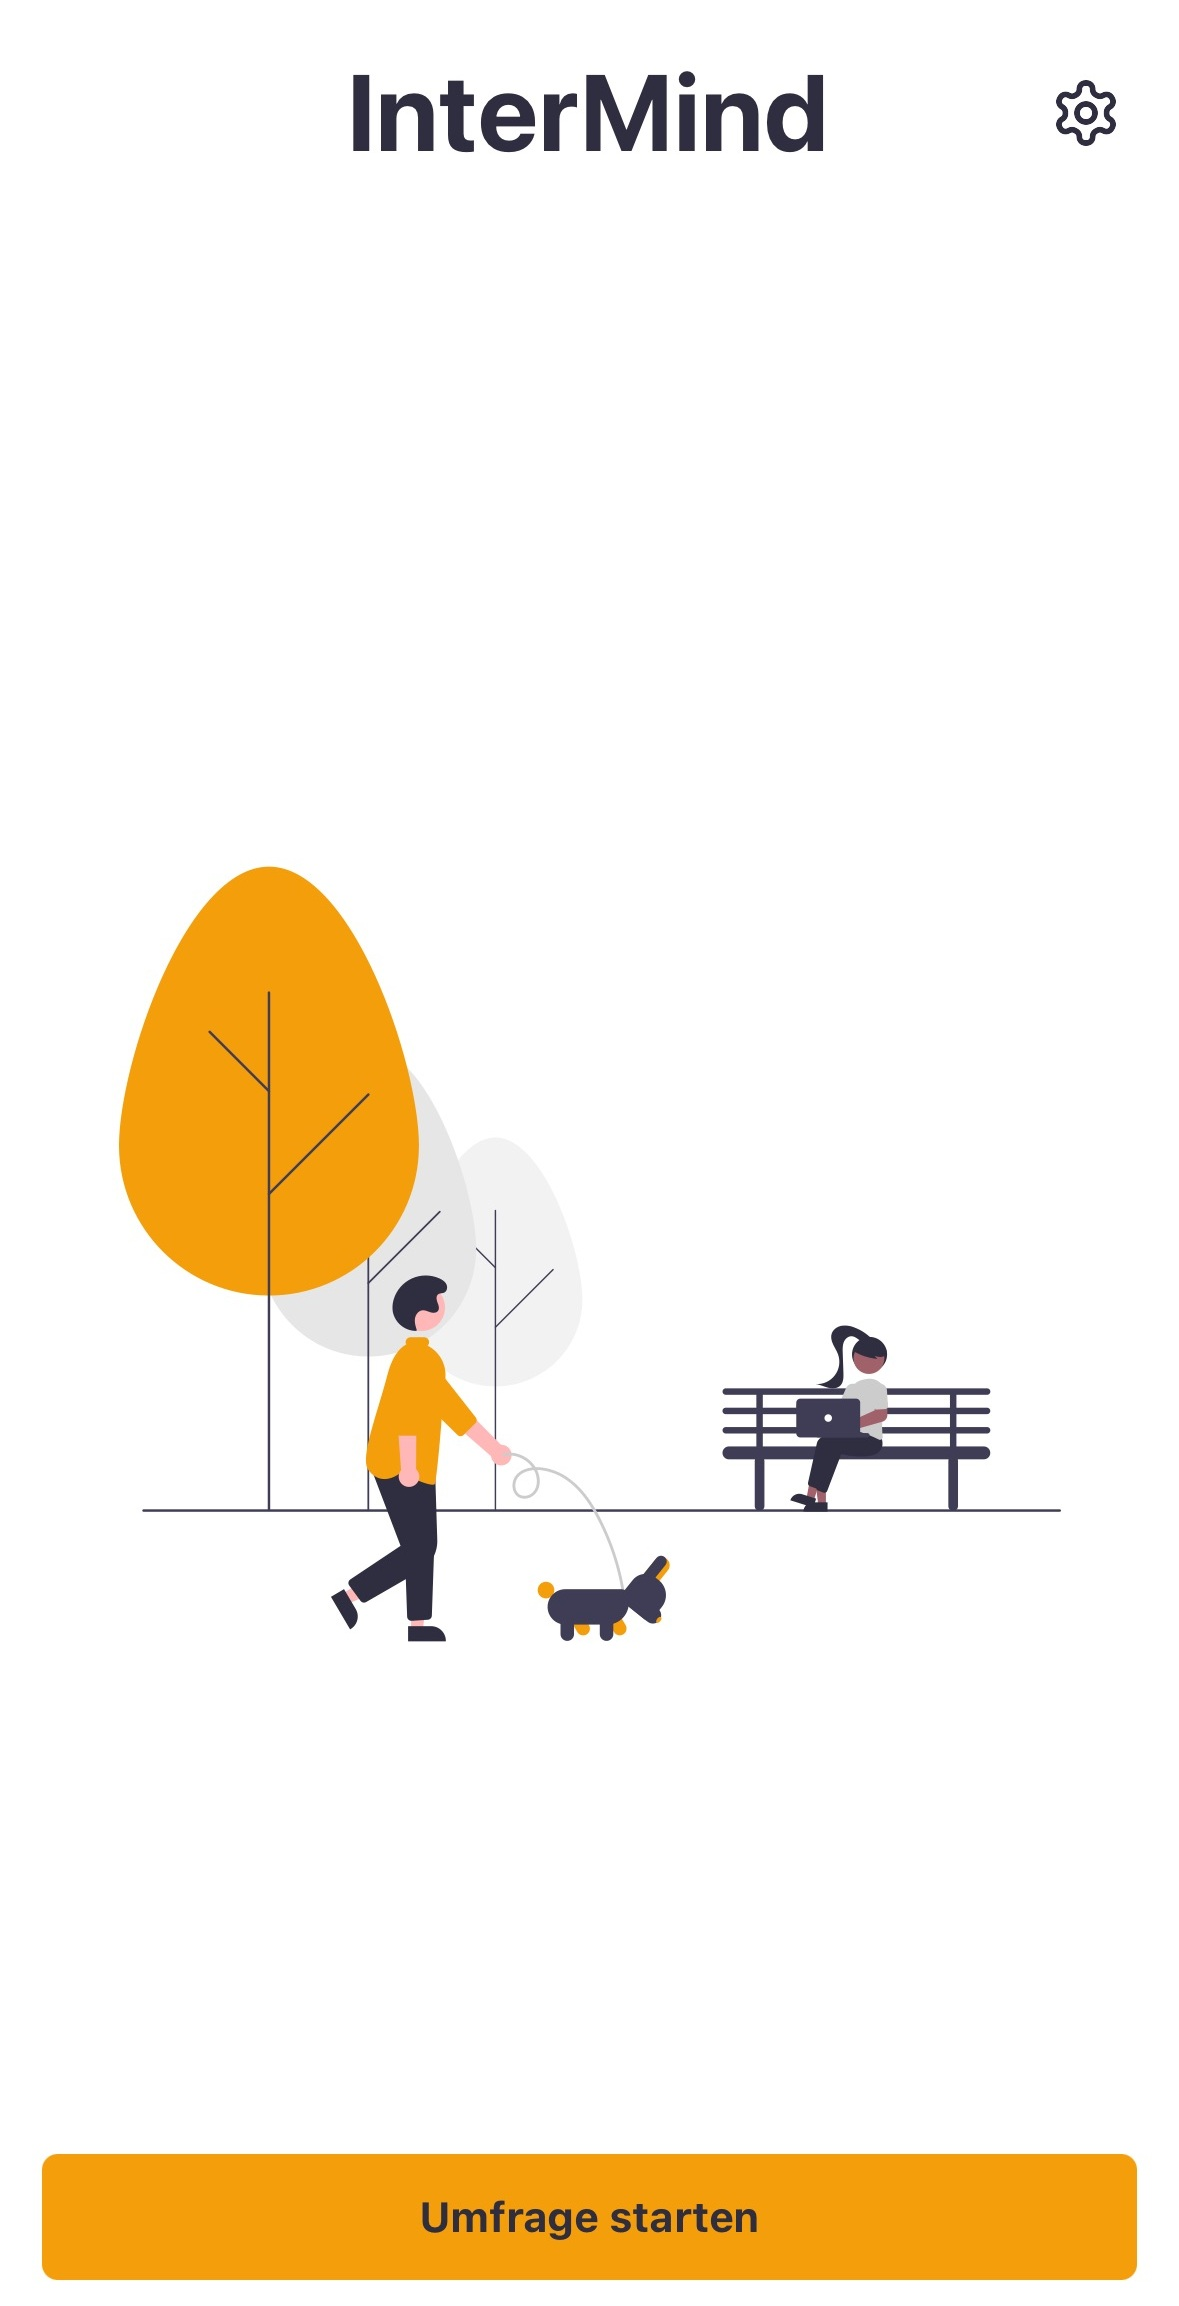
\includegraphics[width=\textwidth]{Arbeit/images/printscreens/startscreen.jpeg}
        \caption{Startbildschirm der App \textit{InterMind}}
        \label{fig:startscreen}
    \end{minipage}
    \hspace{0.1\textwidth}
    \begin{minipage}[t]{0.38\textwidth}
        \centering
        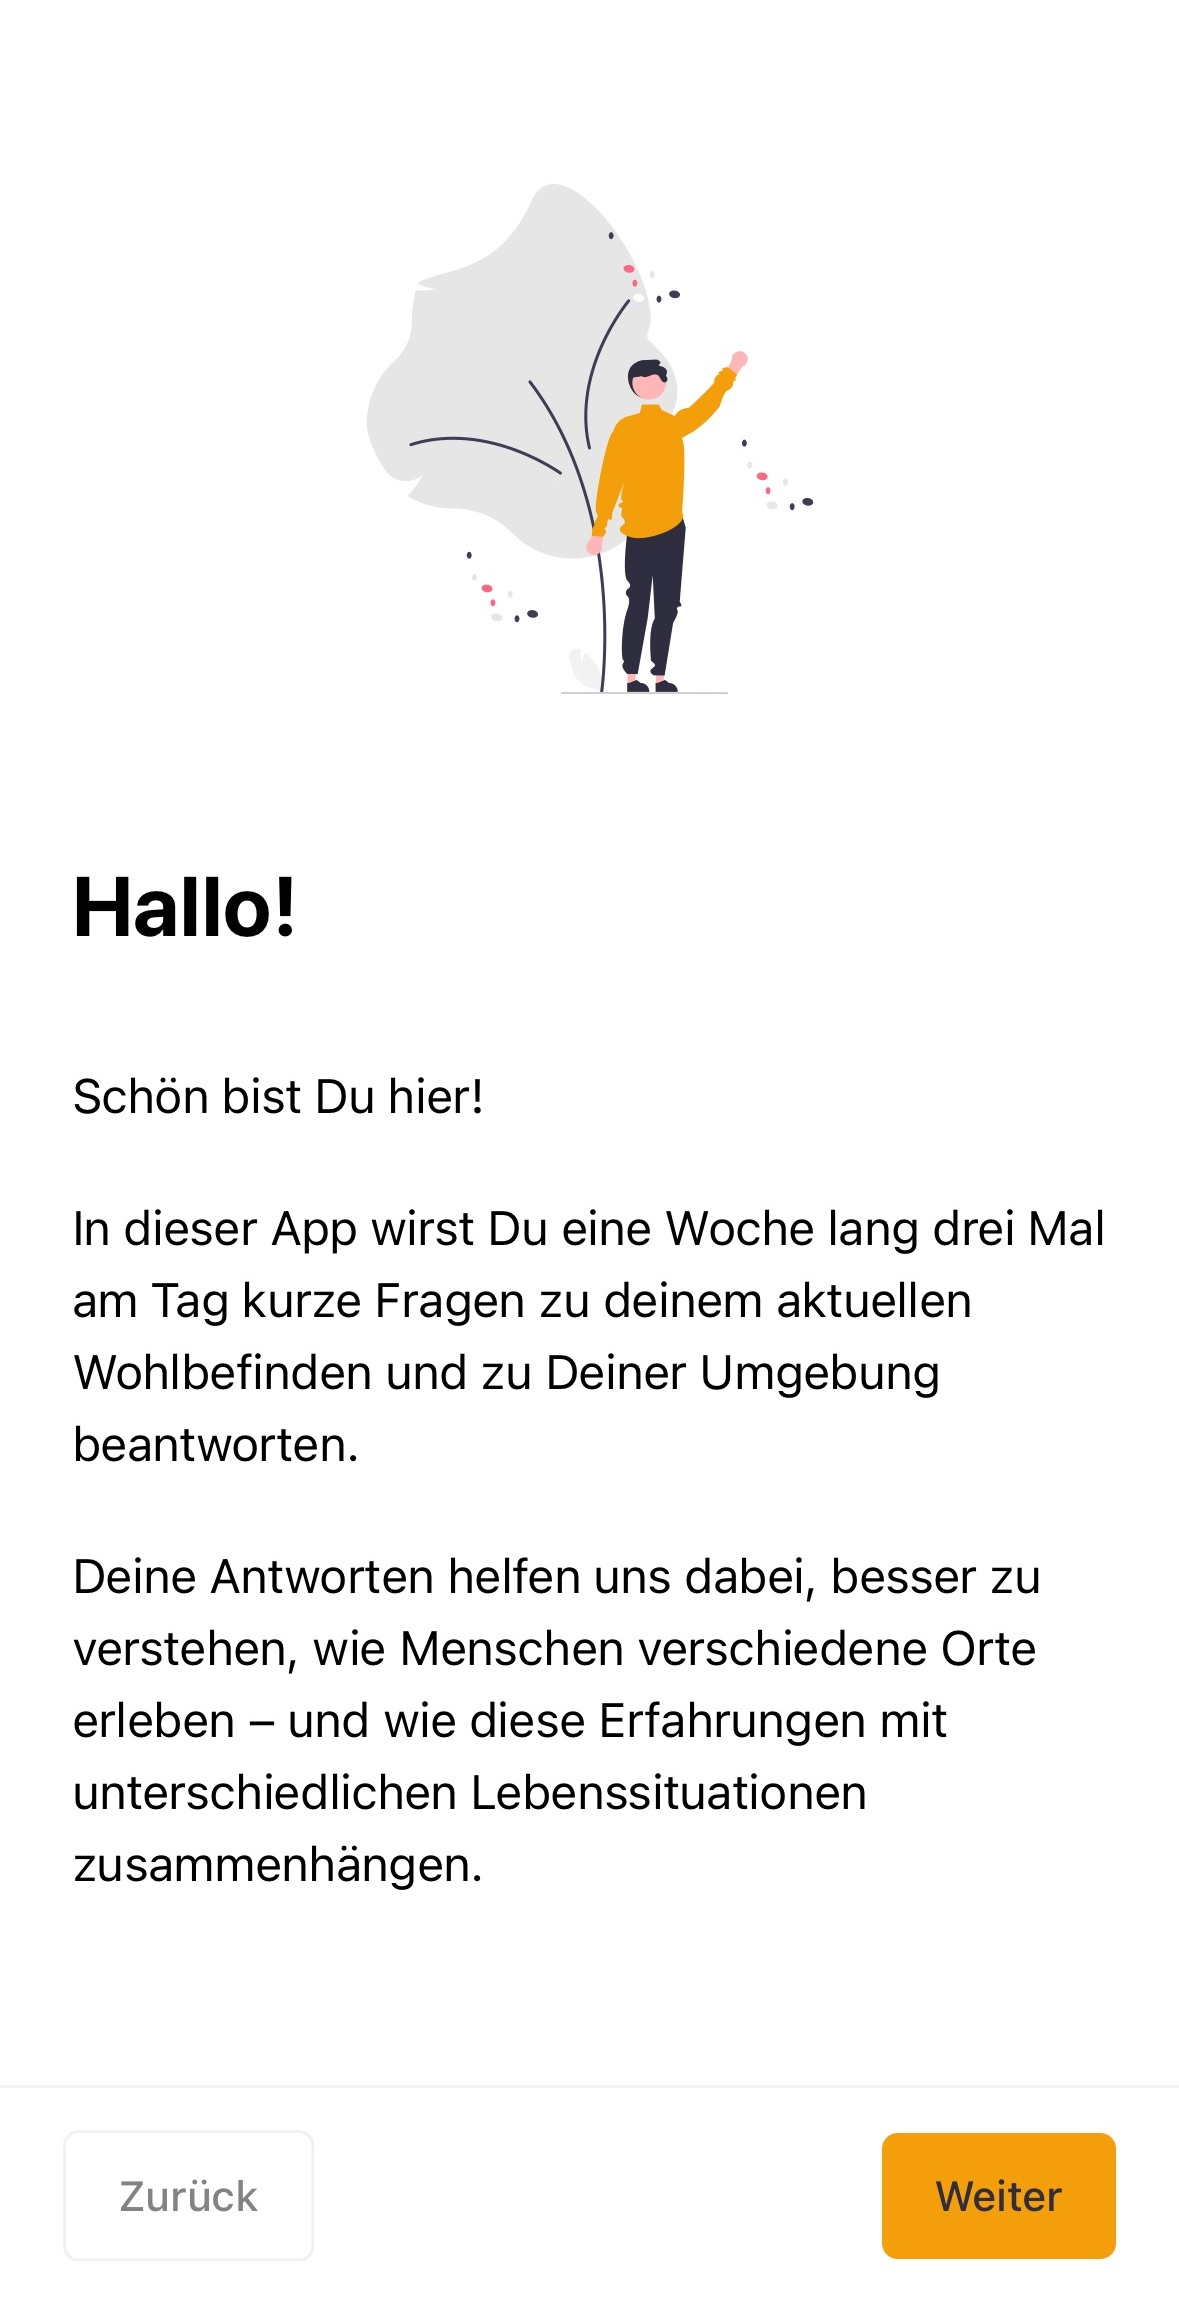
\includegraphics[width=\textwidth]{Arbeit/images/printscreens/welcome.jpeg}
        \caption{Begrüssungstext der App \textit{InterMind}}
        \label{fig:welcome}
    \end{minipage}
\end{figure}


Datenschutz spielte von Beginn an eine zentrale Rolle im Entwicklungsprozess und beeinflusste sowohl die technische Architektur als auch methodische Entscheidungen. Es wird konsequent dem Prinzip \textit{Privacy by Design} gefolgt, das vorsieht, Datenschutzanforderungen bereits bei der Konzeption einer Anwendung mitzudenken und nicht nachträglich zu ergänzen \parencite{cavoukianPrivacyDesign72009}. Ziel ist es, ein hohes Mass an Privatsphäre zu gewährleisten und gleichzeitig volle Transparenz über die Erhebung und Verarbeitung der Daten sicherzustellen.

In der Umsetzung wurde das Prinzip \textit{Privacy by Design} konkret durch technische Massnahmen wie \textit{privacy by architecture} realisiert \parencite{spiekermannEngineeringPrivacy2009}. Die App erfasst keine personenbezogenen Angaben wie Namen, Telefonnummern oder E-Mail-Adressen. Stattdessen wird beim ersten Start automatisch eine gerätegebundene \glsfirst{uuid} generiert, über die alle Daten pseudonymisiert zugeordnet werden. Eine kontinuierliche Ortung findet nicht statt; Standortdaten werden ausschliesslich zum Zeitpunkt einer beantworteten Befragung erhoben.


Die Speicherung der Daten erfolgt auf einem Server in der Schweiz unter Verwendung der Plattform \gls{supabase} und einer \gls{postgresql}-\gls{datenbank}. Eine Zugriffskontrolle auf Zeilenebene (\gls{rls}) stellt sicher, dass jedes Endgerät nur auf die eigenen Daten zugreifen kann. Alle Datenübertragungen zwischen App und Server sind verschlüsselt und erfolgen über authentifizierte Schnittstellen.

Teilnehmende können ihre Datensätze jederzeit direkt über die App löschen. Damit werden sämtliche Einträge, die mit ihrer \gls{uuid} verknüpft sind, dauerhaft entfernt. Die Kontrolle über die eigenen Daten bleibt somit vollständig bei den Nutzer\genderstern innen.

Alle datenschutzrelevanten Aspekte sind in einer eigenen Datenschutzrichtlinie dokumentiert, die über die App sowie auf der Projektwebseite\footnote{\href{https://intermind.ch/privacy-policy.html}{https://intermind.ch/privacy-policy.html}} öffentlich zugänglich ist. Die Richtlinie erläutert zudem die Rechte der Teilnehmenden nach Schweizer Datenschutzgesetz (\gls{dsg}) und der Europäischen Datenschutzgrundverordnung (\gls{dsgvo}).

\vspace{1em}

\begin{figure}[h]
    \centering
    \begin{minipage}[t]{0.38\textwidth}
        \centering
        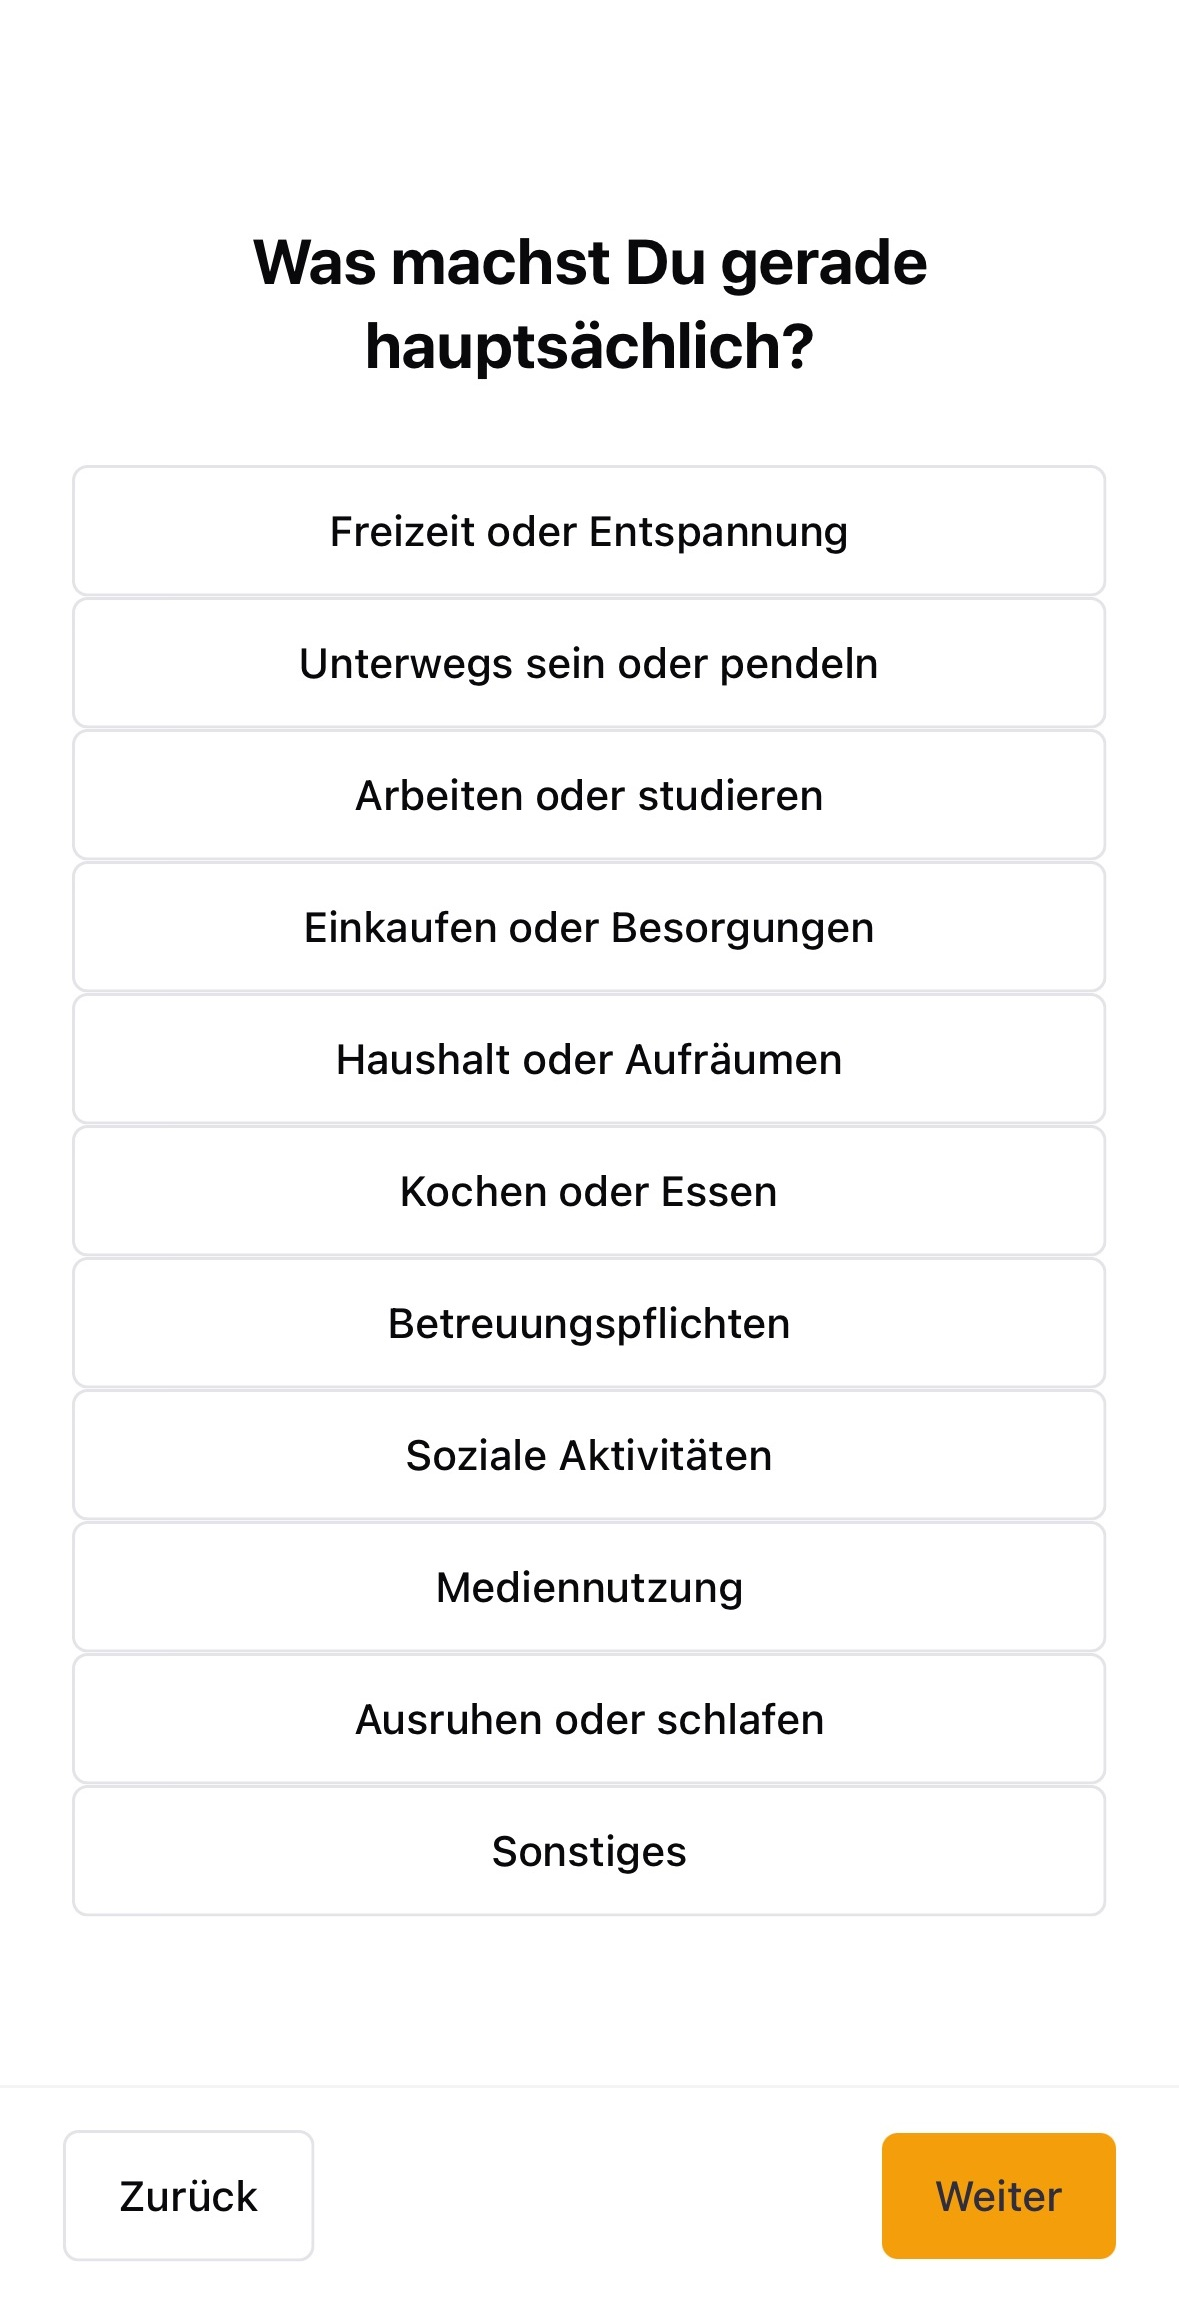
\includegraphics[width=\textwidth]{Arbeit/images/printscreens/beschaeftigung.jpeg}
        \caption{Multiple-Choice-Frage zur aktuellen Beschäftigung}
        \label{fig:beschaeftigung}
    \end{minipage}
    \hspace{0.1\textwidth}
    \begin{minipage}[t]{0.38\textwidth}
        \centering
        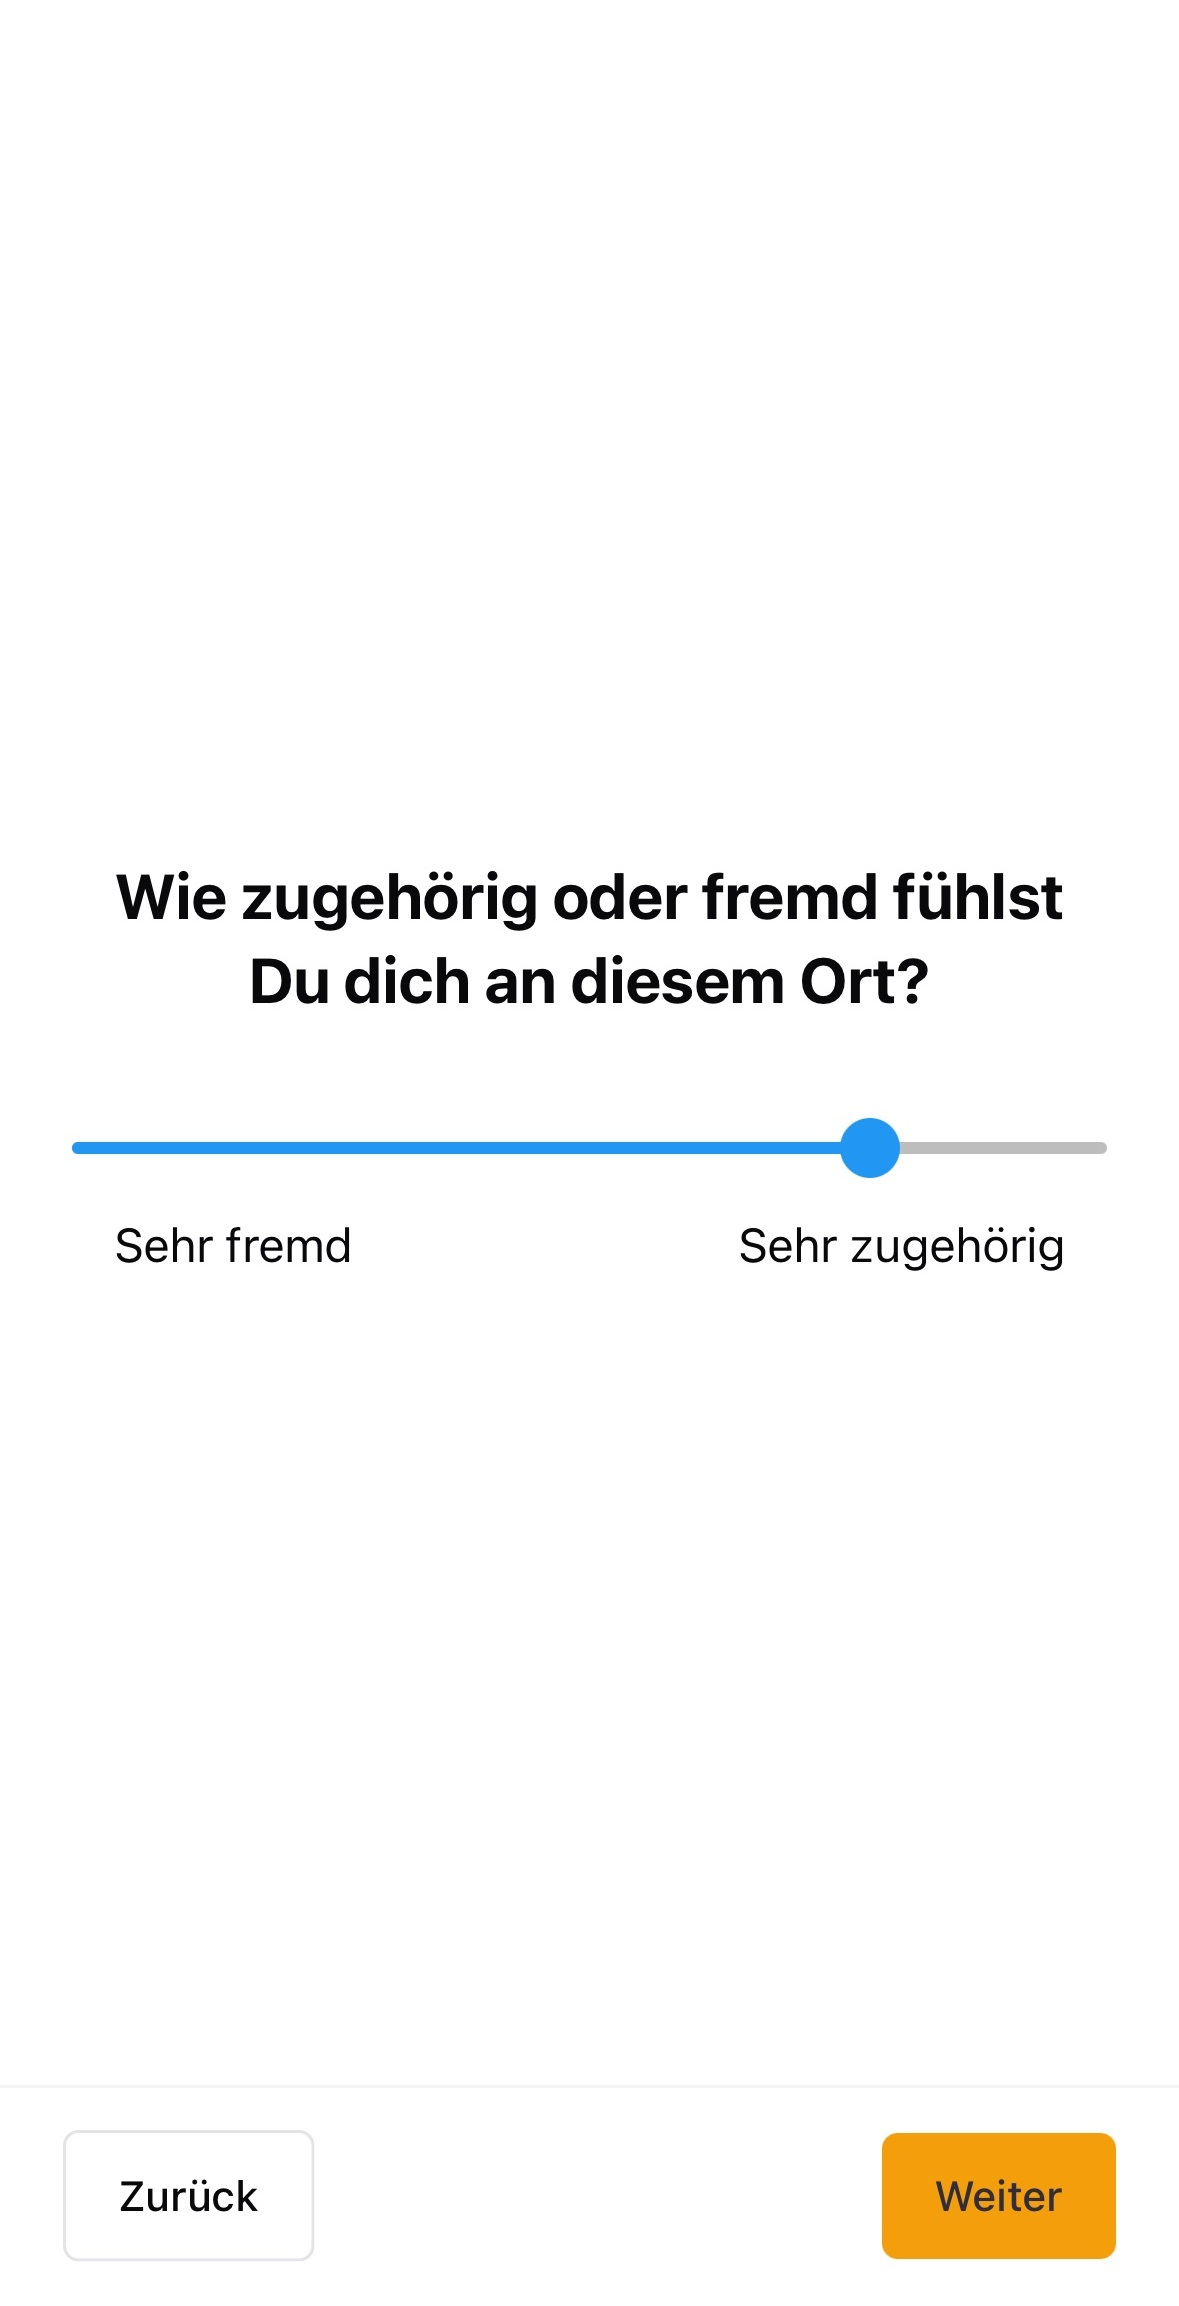
\includegraphics[width=\textwidth]{Arbeit/images/printscreens/zugehoerigkeit.jpeg}
        \caption{Slider-Frage zur sozialen Zugehörigkeit}
        \label{fig:zugehoerigkeit}
    \end{minipage}
\end{figure}


Die technische Umsetzung orientierte sich an etablierten Prinzipien des Software Engineerings \parencite{sommervilleSoftwareEngineering2016} sowie an den zentralen Gestaltungsprinzipien von \gls{solid} \parencite{martinCleanArchitectureCraftsmans2018}. Im Zentrum standen dabei eine saubere Trennung zwischen Anwendungslogik, Datenhaltung und Benutzeroberfläche, eine modulare Struktur der Komponenten sowie eine klare Zuordnung von Verantwortlichkeiten.

Für die Umsetzung wurde das \gls{framework} \gls{reactnative} in Kombination mit der Entwicklungsplattform \gls{expo} gewählt. Diese Entscheidung ermöglichte es, mit einer einheitlichen Codebasis sowohl \gls{ios}- als auch \gls{android}-Geräte zu unterstützen. Dadurch reduzierte sich der Entwicklungsaufwand, während gleichzeitig eine konsistente Benutzererfahrung auf beiden Plattformen sichergestellt werden konnte. Als serverseitige Infrastruktur kam \gls{supabase} zum Einsatz – ein \gls{opensource} \gls{backend}-as-a-Service auf Basis einer relationalen \gls{postgresql}-\gls{datenbank}, das \gls{authentifizierung}, \gls{autorisierung}, Datenspeicherung und sichere Datenübertragung integriert bereitstellt.

Der Fragenkatalog ist nicht im Quellcode verankert, sondern wird dynamisch über eine \gls{json}-Konfigurationsdatei aus der \gls{datenbank} geladen. Dadurch können Inhalte ohne App-Update angepasst werden, was weitestgehend verhindert, dass inkompatible Versionen der App entstehen. Diese Flexibilität erfordert jedoch eine aktive Internetverbindung für das Laden der Befragungsinhalte.

Nach dem erstmaligen Ausfüllen eines Fragebogens berechnet die App automatisch drei individuelle und zufällige Befragungszeitpunkte pro Tag. Diese werden lokal auf dem Gerät gespeichert. Die Zeitpunkte werden täglich zufällig innerhalb von drei Tagesabschnitten (Morgen, Mittag/Nachmittag, Abend) gewählt. Ein Mindestabstand zwischen den einzelnen Befragungen garantiert eine gleichmässige zeitliche Verteilung. Sobald ein Zeitpunkt erreicht ist, erhalten die Teilnehmenden eine Benachrichtigung und haben ab diesem Moment exakt eine Stunde Zeit, um den Fragebogen auszufüllen. Wird der Fragebogen nicht innerhalb dieser Zeitspanne ausgefüllt, verfällt der Slot und die App schickt eine weitere Benachrichtigung beim nächsten geplanten Zeitpunkt.

Das \gls{frontend} wurde minimalistisch und funktional gestaltet, um eine intuitive Nutzung zu ermöglichen und eine möglichst neutrale Darstellung der Fragen sicherzustellen \parencite{rogersInteractionDesignHumancomputer2023}. Die App gliedert sich in drei Hauptbereiche: einen Startbildschirm mit dem nächsten Befragungszeitfenster, den Fragebogenbereich und einen Informations- und Einstellungsbildschirm mit Hinweisen zum Datenschutz. Zur visuellen Unterstützung wurden generische \gls{opensource}-Vektorgrafiken von Katerina Limpitsouni\footnote{\href{https://undraw.co/}{undraw.co/}} verwendet.


\subsection{Von der Simulation zum Alltagstest – Feldtest und Feinschliff}
\label{sec:app_entwicklung_feldtest}

Zur Überprüfung der technischen Funktionsfähigkeit wurde ein zweistufiges Testverfahren durchgeführt, bestehend aus fortlaufenden Tests während der Entwicklung sowie einem abschliessenden internen Pretest. Auf automatisierte Tests wurde verzichtet, da deren Relevanz zu Beginn des Projekts unterschätzt wurde und eine nachträgliche Integration mit erheblichem Aufwand verbunden gewesen wäre. Stattdessen wurde ein manueller, iterativer Testansatz verfolgt. Die App wurde regelmässig mit \glspl{emulator} unterschiedlicher Bildschirmgrössen sowie auf physischen Geräten getestet. Die modulare Struktur der Codebasis sowie die Orientierung an den \gls{solid}-Prinzipien erleichterten dabei die gezielte Überprüfung einzelner Komponenten.

Im Zentrum der technischen Tests standen die dynamische Verarbeitung des Fragenkatalogs, die Datenübertragung an das \gls{supabase}-\gls{backend}, das Verhalten bei instabiler Internetverbindung sowie die lokale Planung von Push-Benachrichtigungen. Letztere erwiesen sich als besonders fehleranfällig, da die ursprüngliche Logik auf Hintergrundprozesse angewiesen war, die von beiden Betriebssystemen aus Effizienzgründen nicht immer zuverlässig gehandhabt werden.

Im Anschluss an die Implementierung wurde ein interner Pretest mit vier Personen durchgeführt. Die Testpersonen erhielten über die offiziellen Plattformen (\gls{testflight} und \gls{googleplayconsole}) Zugang zur App und nutzten diese über einen Zeitraum von zwei Wochen. Ziel war es, zentrale Funktionen unter Alltagsbedingungen zu überprüfen und Rückmeldungen zur allgemeinen Bedienbarkeit zu erhalten. Technische Aspekte wie das Verhalten beim ersten App-Start, die Stabilität der Datenerfassung und die Darstellung auf unterschiedlichen Geräten wurden dabei gezielt beobachtet.

Die Ergebnisse des Tests führten zu mehreren Anpassungen der App. So wurde bspw. die Logik zur Planung der Slots und Benachrichtigungen grundlegend überarbeitet: Anstelle von Hintergrundprozessen werden nun sämtliche Befragungszeitpunkte direkt nach dem Abschluss der ersten Befragung berechnet und lokal gespeichert. So konnten sämtliche Hintergrundprozesse eliminiert werden.

Zusätzlich wurden verschiedene kleinere Anpassungen an der Benutzeroberfläche vorgenommen, insbesondere im Hinblick auf die Darstellung von \gls{ui}-Elementen auf kleineren Bildschirmen sowie die Positionierung und Lesbarkeit von Slider-Beschriftungen. Diese Optimierungen trugen dazu bei, die visuelle Konsistenz der App auf verschiedenen Geräten zu verbessern.

\subsection{App-Veröffentlichung – Prozesse, Plattformen, Abhängigkeiten}

Um die entwickelte App für die eigentliche Datenerhebung nutzen zu können, wurde eine Veröffentlichung über die offiziellen App-Stores von Apple (iOS) und Google (Android) angestrebt. Beide Plattformen stellen dabei unterschiedliche technische, administrative und finanzielle Anforderungen, die den Veröffentlichungsprozess massgeblich beeinflussten.

Die Veröffentlichung im Apple App Store setzte zunächst den Erwerb einer kostenpflichtigen Entwicklerlizenz voraus, für die eine jährliche Gebühr von CHF 100 zu entrichten war. Nach erfolgreicher Einrichtung dieses Entwicklerkontos wurde die App zur Veröffentlichung eingereicht, allerdings von Apple zunächst nicht für eine finale Veröffentlichung im regulären App Store zugelassen. Als Begründung wurde angegeben, die App weise zu wenig inhaltlichen Mehrwert auf – eine Entscheidung, die aus Sicht der Entwicklung nur schwer nachvollziehbar war. Der Prüfprozess bei Apple ist zum Zeitpunkt des Abschlusses dieser Arbeit noch nicht vollständig abgeschlossen. Dennoch konnte die App über Apples eigene Plattform für öffentliche Beta-Tests (\gls{testflight}) bereitgestellt werden, sodass Teilnehmende der Studie über einen Link Zugang zur App erhielten.

Im Gegensatz dazu verlangte Google für eine Veröffentlichung im Android Play Store keine laufenden Lizenzkosten. Allerdings stellte Google die Bedingung, dass vor einer offenen Betaversion zunächst ein geschlossener Test mit mindestens 20 Personen über einen Zeitraum von zwei Wochen durchgeführt werden musste. Da es innerhalb des zeitlichen Rahmens dieser Bachelorarbeit nicht möglich war, eine ausreichende Anzahl Testpersonen mit Android-Geräten zu rekrutieren, wurde hierfür ein externer Dienstleister in Anspruch genommen, welcher diesen erforderlichen Test für eine Gebühr von CHF 30 durchführte. Nach erfolgreichem Abschluss dieses Tests wurde die App im Play Store als offene Beta veröffentlicht und war somit öffentlich verfügbar.

Darüber hinaus verlangten beide Plattformen, dass eine öffentlich zugängliche Datenschutzrichtlinie zur Verfügung steht. Zu diesem Zweck wurde eine Website\footnote{\href{https://intermind.ch/privacy-policy.html?lang=de}{intermind.ch/privacy-policy}} eingerichtet, auf der die vollständige Datenschutzerklärung einsehbar ist. Die Kosten hierfür beliefen sich auf einmalig CHF 10 für die Domainregistrierung; Hosting-Kosten entstanden keine zusätzlichen, da auf bereits bestehende Infrastruktur zurückgegriffen wurde.

\begin{figure}[h]
    \centering
    \begin{minipage}[t]{0.38\textwidth}
        \centering
        
\includegraphics[width=\textwidth]{Arbeit/images/printscreens/fragen_zu_dir.jpeg}
        \caption{Überleitungsbildschirm zu den einmaligen Fragen}
        \label{fig:ueberleitungsbildschirm}
    \end{minipage}
    \hspace{0.1\textwidth}
    \begin{minipage}[t]{0.38\textwidth}
        \centering
        
\includegraphics[width=\textwidth]{Arbeit/images/printscreens/offen_unwohl.jpeg}
        \caption{Offene Textfrage zu weiteren Gründen für Unwohlsein an diesem Ort}
        \label{fig:offene_textfrage}
    \end{minipage}
\end{figure}

\subsection{Eigenständig, aber nicht unabhängig – Entwicklung im Plattformzeitalter}

Die Entwicklung von \textit{InterMind} war mein erstes grösseres Projekt in \gls{typescript} und mit \gls{reactnative}. Die Umstellung vom strikt objektorientierten Denken in \gls{java} auf den dynamischeren, komponentenbasierten Ansatz war anspruchsvoll, aber enorm lehrreich. Insbesondere das konsequente Anwenden der \gls{solid}-Prinzipien half dabei, die Struktur der Anwendung nachvollziehbar zu halten – gerade in einem neuen Ökosystem. Die App funktioniert stabil, sieht gut aus, und hat ihren Zweck erfüllt.

Trotz einer bewussten Orientierung an Prinzipien wie \gls{solid} und einem grundlegenden Architekturkonzept zeigte sich im Verlauf der Entwicklung, dass eine noch systematischere Auseinandersetzung mit der Softwarearchitektur hilfreich gewesen wäre. Zwar wurde auf eine modulare Struktur geachtet, viele Designentscheidungen wurden jedoch eher situativ getroffen und nicht im Sinne eines übergeordneten Gesamtdesigns immer wieder überprüft. Gerade im weiteren Projektverlauf wäre es sinnvoll gewesen, gezielt zu früheren architektonischen Überlegungen zurückzukehren und diese zu reflektieren oder anzupassen.

Methoden wie \emph{Test-Driven Development} hätten diesen Prozess zusätzlich stützen können, indem sie klare Schnittstellen und Verantwortlichkeiten frühzeitig erzwingen. Auch der Aufbau automatisierter Tests und eine kontinuierlich integrierte Codeanalyse hätten dazu beigetragen, Fehlerquellen frühzeitig zu identifizieren und die langfristige Wartbarkeit der Anwendung zu verbessern. Viele kleinere Schwächen im Code wurden zwar pragmatisch behoben, ein strukturierteres Qualitätsmanagement hätte jedoch die Notwendigkeit späterer Refactoring-Prozesse deutlich reduziert.

In diesem Sinne reiht sich die App auch in eine typische Dynamik vieler \gls{opensource}-Projekte ein: Sie wurde aus einem konkreten Forschungsbedarf heraus entwickelt, funktioniert zuverlässig, ist öffentlich dokumentiert – aber nicht in jedem Teilbereich optimal strukturiert. Durch die Offenlegung des Quellcodes besteht jedoch die Möglichkeit, dass andere Entwickler\genderstern innen auf dieser Grundlage aufbauen, Verbesserungsvorschläge einbringen oder eigene Erweiterungen umsetzen.

Die Erfahrungen rund um die Veröffentlichung in den App Stores hat zentrale Spannungsfelder digitaler Infrastruktur deutlich gemacht. Obwohl die App funktional einsatzbereit war und über TestFlight bzw. den Play Store zugänglich gemacht werden konnte, blieb die reguläre Veröffentlichung im Apple App Store aufgrund einer intransparenten Ablehnung verwehrt.

Solche Prozesse offenbaren strukturelle Abhängigkeiten, die weit über dieses Projekt hinausgehen: Zwei gigantische multinationale Tech-Konzerne kontrollieren in weiten Teilen den Zugang zu digitaler Infrastruktur. Dabei wirken sie zugleich als Regelsetzer, Infrastrukturbetreiber und ökonomische Gatekeeper. Diese doppelte Rolle ist nicht demokratisch legitimiert, aber mit erheblicher Lenkungsmacht verbunden. Gerade nicht-kommerzielle, experimentelle oder aktivistische Projekte sind von diesen Kontrollmechanismen besonders betroffen, da sie sich nicht ohne Weiteres den geforderten Verwertungslogiken oder Standardprozessen unterwerfen.

Auch wenn Open-Source-Prinzipien allein diese strukturellen Hürden nicht auflösen können, war die Entscheidung zur Veröffentlichung des Quellcodes dennoch zentral: Sie schafft Transparenz, ermöglicht Weiterentwicklung und signalisiert ein bewusstes Gegenmodell zu proprietären, intransparenten Systemen. Gleichzeitig offenbart sich hier ein grundlegendes Spannungsfeld: Die offene, zugängliche und gemeinschaftsorientierte Logik von \gls{opensource}-Software steht in einem scharfen Kontrast zu den geschlossenen, marktkontrollierten Strukturen kommerzieller Distributionsplattformen. Wer eine App entwickeln und öffentlich zugänglich machen will, ist faktisch gezwungen, sich diesen Plattformen zu unterwerfen.

Die Arbeit an der App war dabei nicht nur funktional motiviert, sondern auch von der Erfahrung getragen, ein eigenes digitales Werkzeug gestalten zu können – mit all seinen Herausforderungen, aber auch mit dem unmittelbaren Lernerfolg und der Freude am konkreten Entstehungsprozess. Gerade vor dem Hintergrund einer zunehmend von privatwirtschaftlichen Plattformen dominierten digitalen Infrastruktur bleibt die Fähigkeit, eigene Werkzeuge zu entwickeln, ein wichtiger Akt technischer Aneignung.